\pagestyle{fancy}
\chapter{Definición del proyecto}
En este primer capítulo se acerca al lector a las motivaciones que han dado forma al proyecto fin de carrera. Para ello se explicará el concepto de los móviles de tipo smartphone, describiendo su situación actual del mercado y las distintas plataformas existentes para el desarrollo de aplicaciones, en concreto para videojuegos.
\newline

Un segundo punto a tratar, será la evolución de los videojuegos durante el trascurso de los años, desde un enfoque de hardware y software, sin olvidar las implicaciones de ser desarrollados en smartphones.
\newline

Para finalizar el capítulo se describirán los objetivos que se pretenden alcanzar en la realización del proyecto.
\newpage

\section{Motivación del proyecto}

Lejos estamos de los años 90 cuando la segunda generación de móviles comenzaba a inundar los mercados. Hoy en día es difícil encontrar a alguien que no tenga uno, es más, se han convertido en un utensilio indispensable en la vida cotidiana de las personas. Los teléfonos móviles han ido evolucionando hasta convertirse en lo hoy conocemos como \emph{smartphone} o \emph{teléfonos inteligentes}. 
\\

Esta denominación se debe a una capacidad de computación avanzada, que unida a su conectividad, nos permite trasladar la mayoría de las tareas que realizamos en computadoras personales como son gestionar correos, ver vídeos, escuchar música, jugar a videojuegos\ldots\ a nuestro ordenador de bolsillo, el smartphone.
\newline

\begin{figure}[h]
	\centering
	\subfloat[Ventas mundiales smarthpones]{
	          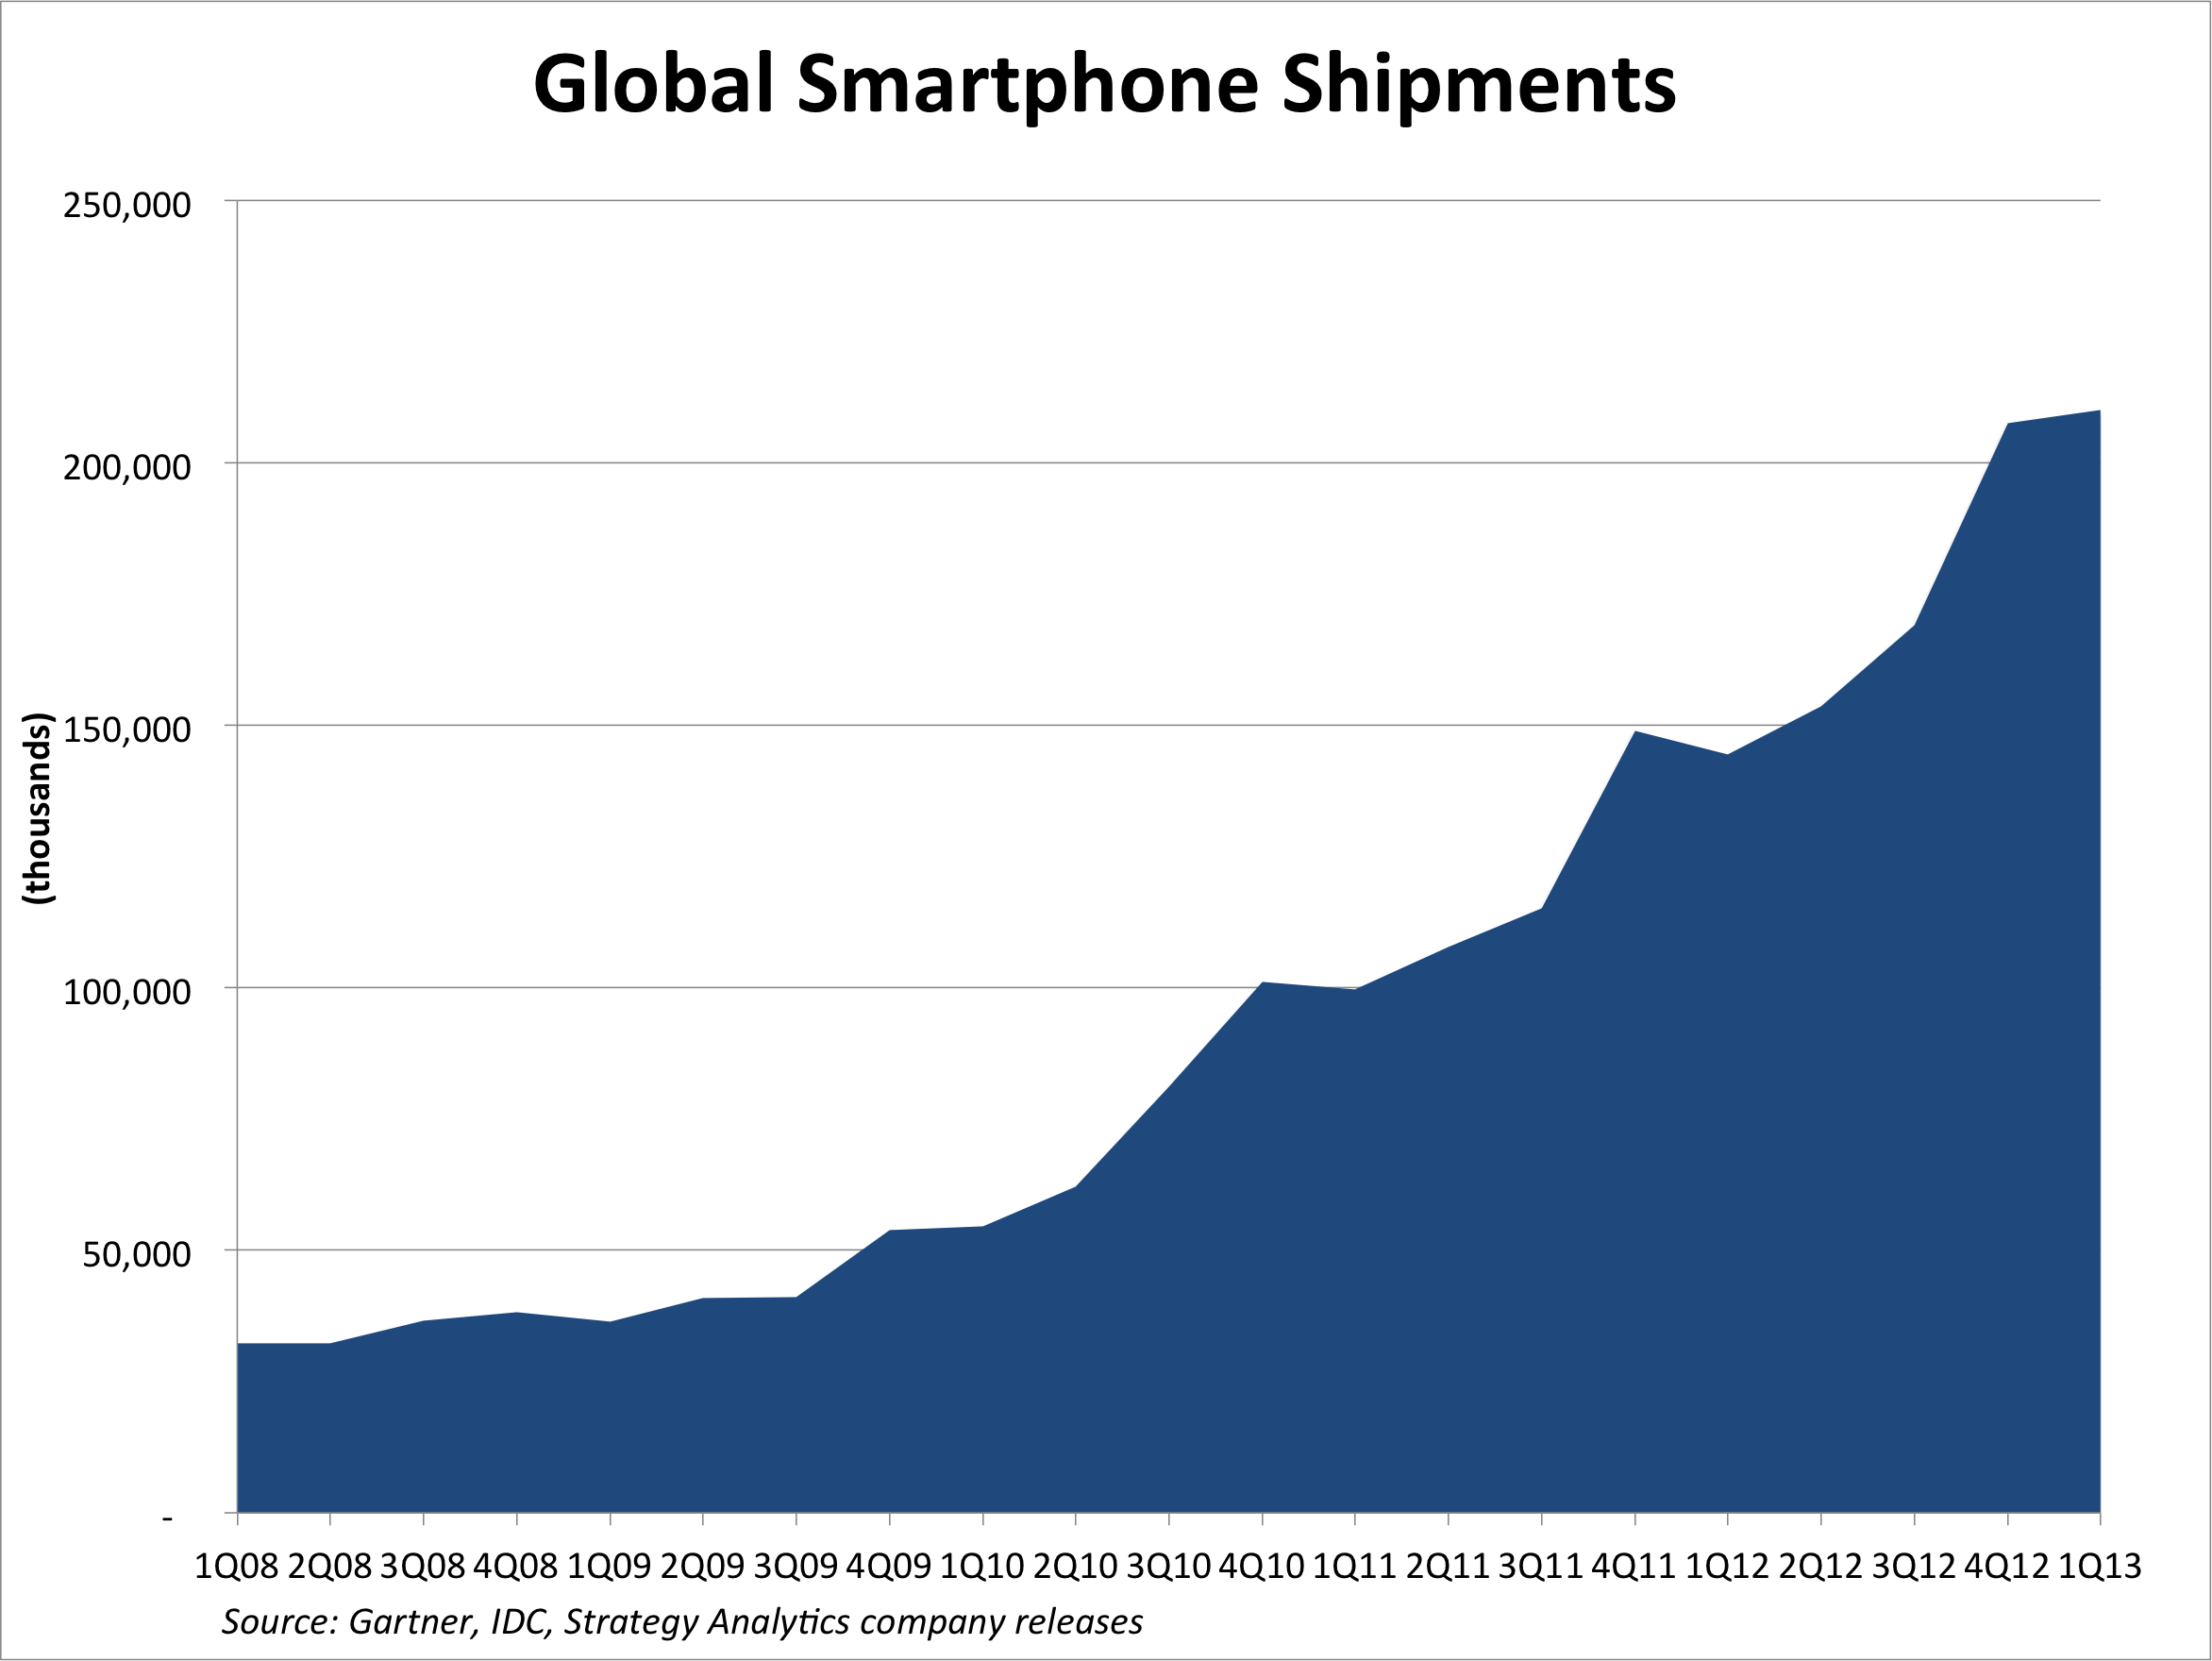
\includegraphics[height=46mm]{imagenes/capitulo1/img1.png}
	}
	\subfloat[Distribución mundial]{
	          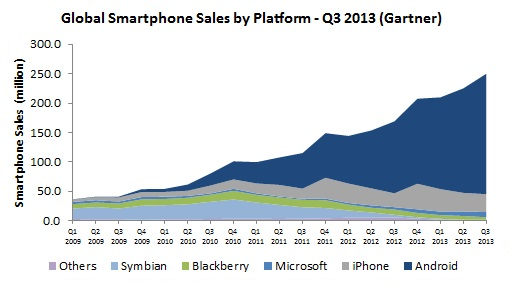
\includegraphics[height=46mm]{imagenes/capitulo1/img3.jpg}
	}

	\subfloat[Distribución en EEUU]{
	          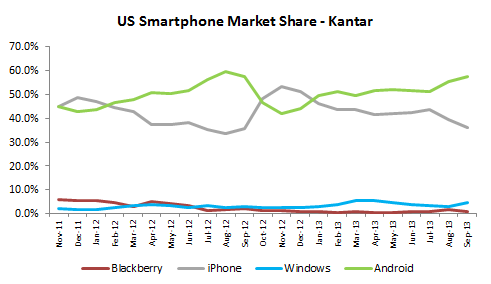
\includegraphics[height=42mm]{imagenes/capitulo1/img4.png}
	}
	\subfloat[Distribución en España]{
	          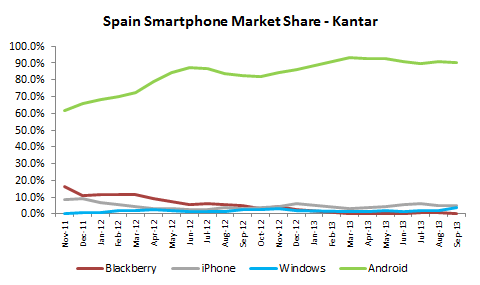
\includegraphics[height=42mm]{imagenes/capitulo1/img2.png}
	}
	\caption{Situación actual de los smartphones}
\end{figure}

Al observar en la gráfica ``a'' de la figura 1.1, podemos ver que el número de ventas de móviles se incrementan año tras año. Debido a su alto coste, la estrategia de mercado se está centrando en desarrollar este tipo de dispositivo low-cost, con un menor coste, para que estén al alcance de todos los bolsillos. El objetivo de esta estrategia es doblar la venta de smartphones de bajo presupuesto de forma anual hasta 2016, pasando de 4 millones de unidades en el año 2010 a unas 311 millones 6 años después.
\newline

En el resto de los gráficos de la figura 1.1 se muestra la distribución de las principales plataformas ejecutadas en los smartphones a nivel mundial, en Estados Unidos y en España. Cabe destacar que la plataforma Symbian, de Nokia, ha desaparecido casi por completo. A nivel mundial es un mercado dominado por Android. Ocurre lo mismo en España pero en Estados Unidos comparte el mercado junto con iPhone.
\newline

Tras realizar un pequeño análisis de las dos plataformas dominantes, se ha llegado a las siguientes conclusiones:
\begin{itemize}
\item Tanto Android como iPhone ofrecen un marco de trabajo en una primera fase estable y suficientemente evolucionado para el desarrollo de un proyecto de fin de carrera.
El desarrollo sobre IPhone implica unos gastos superiores respecto a Android debido a temas de licencias, coste del dispositivos y software necesario.
\item El tiempo requerido en el desarrollo sobre un IPhone es menor que en Android. Esta diferencia radica en que IPhone esta soportado en un pequeño conjunto de dispositivos muy reducido, tan sólo los productos ofrecido por la compañía Apple, mientras que en Android existen una gran variedad de  dispositivos con características dispares.
Por este motivo, un programa desarrollado en Android ha de ser probado en un mayor número de dispositivos móviles, lo que conlleva un mayor tiempo de pruebas.
\item El precio de un dispositivo móvil con un sistema Android y las características de aceleración gráfica 3D por hardware, están dentro del presupuesto personal  del proyecto.
\end{itemize}

\begin{figure}[h]
	\centering
        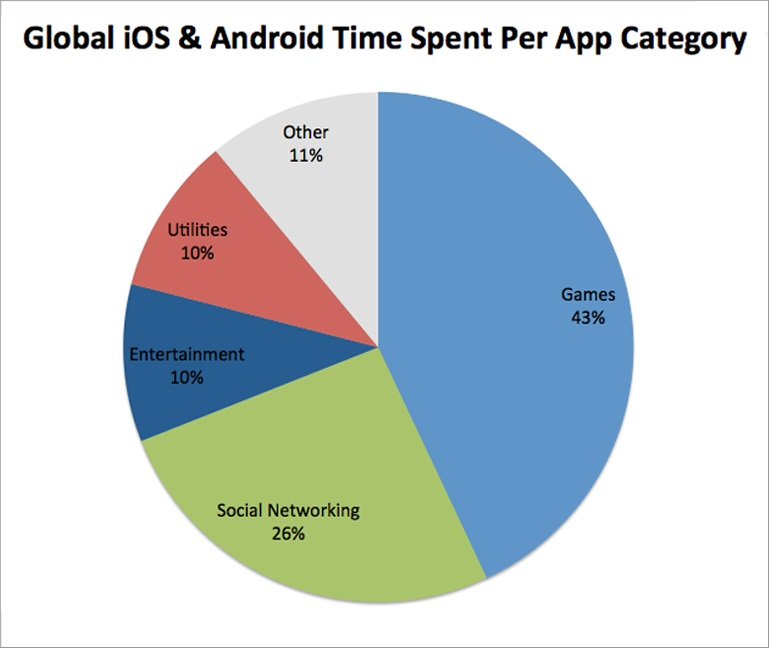
\includegraphics[height=55mm]{imagenes/capitulo1/img5.jpg}
	\caption{¿Para qué usamos los smartphones?}
\end{figure}

La situación descrita suscita un interés especial en adquirir un mayor conocimiento en el desarrollo de aplicaciones para smartphones Android. En la figura 1.2 se muestran un diagrama con las facetas en las que más tiempo empleamos cuando manejamos un smarthpone, lo que nos da una idea de las aplicaciones típicas en un dispositivo de estas características. 
\newline

Hemos de destacar el gran porcentaje de tiempo que dedicamos jugando con el smartphone, lo que justifica que el desarrollo de videojuegos se está convirtiendo en un nuevo nicho de mercado para las empresas. Actualmente existen varios framework de desarrollo de videojuegos con aspecto gráfico tridimensional para Android, el más famoso es Unity 3D. Sin embargo, esta situación era muy distinta cuando comenzó el proyecto, ya que no existía ningún framework o los que existían era muy precarios.
\newline 

Debido a la situación del mercado de los smartphone respecto a la creación de videojuegos con gráficos en 3D, surge en forma de proyecto de fin de carrera, la idea de dar respuesta a la pregunta que hizo que estudiara ingeniería informática años atrás, esa pregunta es:
\begin{center}
\texttt{¿Cómo se hace un videojuego?}
\end{center}

El juego elegido es Pacmania, una versión que simula las tres dimensiones y que la empresa Nanco desarrolló en 1988 basándose en una versión anterior en 2D llamada Pacman, conocida popularmente como comecocos. Se ha decidido implementar este videojuego ya que no existe ninguna versión parecida en Android, tan sólo una versión en 2D. En los siguientes gráficos podemos ver la versión actual para Android del juego Pacman junto con la versión de PC del juego Pacmania.

\begin{figure}[h]
		\centering
		\subfloat[Pacmania (PC)]{
		          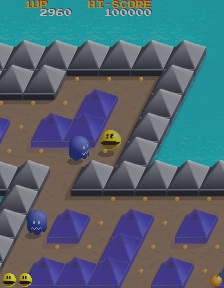
\includegraphics[height=6.5cm]{imagenes/capitulo1/PacmanPC.jpg}
		}
		\subfloat[Pacman (Android)]{
		          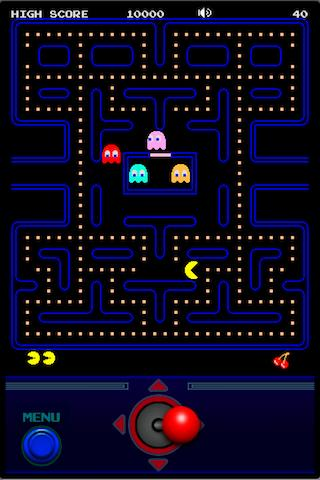
\includegraphics[height=6.5cm]{imagenes/capitulo1/PacmanAndroid.jpg}
		}
\end{figure}
	

\section{Evolución de los videojuegos}

La evolución de los videojuegos puede ser vista desde dos prismas bien diferenciados. Podemos hablar de cómo se han ido adaptando los formatos con los cuales se presentan al mercado, por ejemplo en máquinas recreativas, consolas\ldots\ Otra forma de ver esta evolución es centrándonos en las características de los videojuegos como por ejemplo el aspecto visual, conectividad\ldots\ 
\newline

A continuación vamos a detallar la evolución desde ambos puntos de vista, no sin antes mencionar un aspecto a tener en cuenta. Un cambio de formato puede tener implicaciones directas sobre las características del videojuego, por ejemplo, la diferencia de capacidad de procesamiento entre consolas y dispositivos móviles conlleva una perdida de calidad gráfica.
\newline

\subsection{Evolución de los formatos}

Actualmente el concepto de videojuego ha sido asimilado por la sociedad, cualquiera sabe qué es un videojuego, incluso han dejado de ser un producto exclusivo para adolescentes. Si nos remontamos a la década de los 40, la palabra videojuego aún no existía. En esta década se crean las primeras computadoras de la historia como Zuse, Colossus y ENIAC\ldots\ pero fue en 1949 cuando el laboratorio de Matemáticas de la Universidad de Cambridge presenta EDSAC, una computadora que no sólo se utilizó para realizar cálculos matemáticos. En 1952 Alexander S. Douglas construye sobre ella el videojuego Nought and Crosses, también llamado OXO. En España dicho juego es conocido como las tres en raya y permitía enfrentar a un jugador humano contra la máquina, visualizando el tablero sobre una pantalla de tubo de rayos catódicos.
\newline

\begin{figure}[!h]
	\centering	
	\subfloat[OXO]{
	          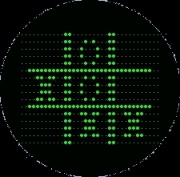
\includegraphics[height=45mm]{imagenes/capitulo1/oxo.jpg}
	}
	\subfloat[Tennis for two]{
	          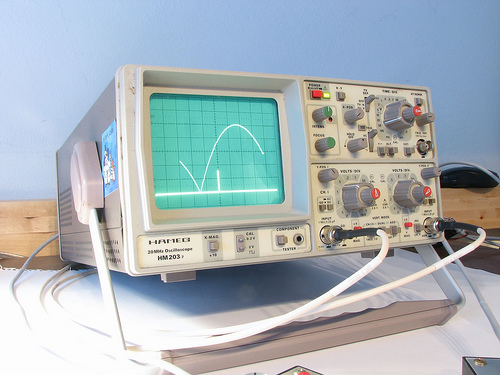
\includegraphics[height=45mm]{imagenes/capitulo1/tennis4two.jpg}
	}
	\caption{Los primeros videojuegos caseros que se crearon}
\end{figure}

En 1958, Will Higinbothamen en el laboratorio nacional de Brookhaven, simuló en un osciloscopio un partido de tenis. No estaba dotada de ningún tipo de inteligencia por lo que no se podía jugar contra la máquina y se necesitaban dos jugadores. Cada uno de ellos manejaba una especie de mando que tenía una pequeña rueda para indicar el ángulo de golpeo y un botón para golpear la pelota con una raqueta invisible. 
\newline

En 1961 unos estudiantes del Instituto de Tecnológico de Massachusetts (MIT), Steve Russell entre ellos, construye SpaceWar, un videojuego donde dos naves espaciales y armadas tenían que destruirse mientras evitaban la fuerza gravitatoria de una estrella. Tras pasarse horas jugando a SpaceWar, en 1971 Rusell finalmente decidió comercializarlo con el nombre ``Computer Space'', lo que dio origen a la primera máquina recreativa. 
\newline

Sin embargo, la difusión en el mercado de Computer Space fue mucho menor que PONG de Atari, la cual simulaba el juego del ping-pong. Esta segunda máquina recreativa salió al mercado un año más tarde, pero debido a que su difusión fue mucho mayor es considerada como la primera máquina recreativa. 
\newline

\begin{figure}[h]
	\centering	
	\subfloat[Pong]{
	          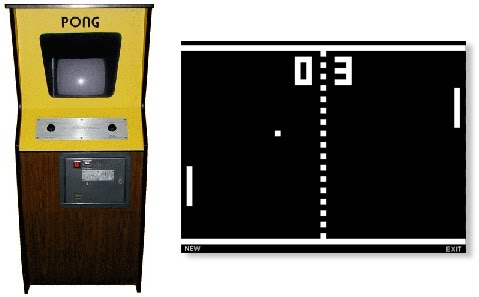
\includegraphics[height=45mm]{imagenes/capitulo1/Pong.jpg}
	}
	\subfloat[Computer Space]{
	          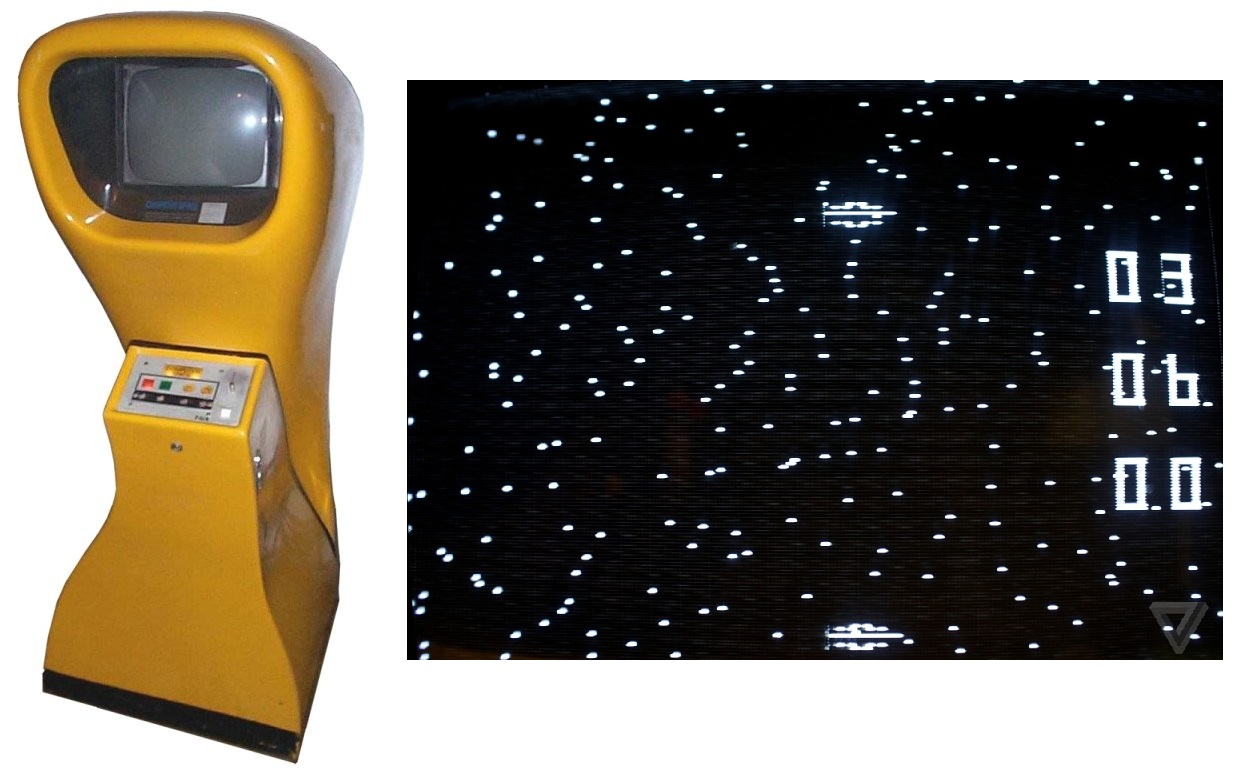
\includegraphics[height=45mm]{imagenes/capitulo1/ComputerSpace.jpg}
	}
	\caption{Los primeras máquinas recreativas}
\end{figure}

Pronto surgieron nuevas máquinas recreativas, algunas de ellas son King Kong, Pacman, Tetris, Super Mario Bros\ldots\ Los adolescentes acudían a un nuevo tipo de negocio, los salones recreativos, donde insertando una moneda podían jugar una partida al videojuego deseado. Este fue el comienzo de la industria de los videojuegos. 
\newline 

Con el trascurso de los años, fueron evolucionando en las temáticas, el aspecto visual y se hicieron más interactivos con la inclusión de nuevos periféricos como volantes, guitarras, cámaras que detectan el movimiento, etc. 
\newline 

En 1972 la industria de los videojuegos daba sus primeros pasos en los hogares con la creación de las primera generación de consolas. Un gran salto que  trasladaba la diversión de los salones recreativos al salón de casa. 
\newline
A continuación se muestra una tabla con las principales consolas que han salido al mercado y a que generación pertenecen.

\begin{figure}[h]
	\centering
         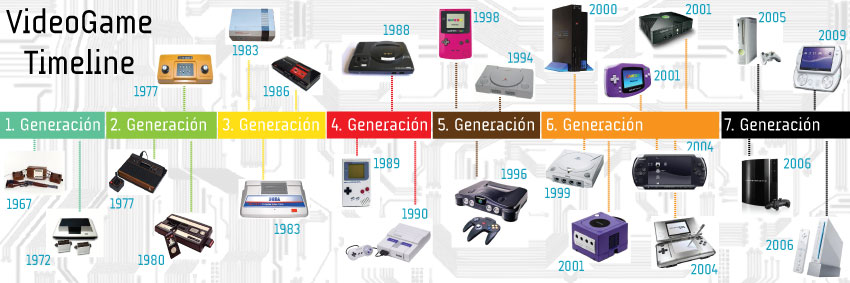
\includegraphics[width=14cm]{imagenes/capitulo1/consolas.jpg}
\end{figure}

Durante las distintas generaciones de consolas han existido intentos, con mayor o menor acierto, de hacerlas portátiles, ejemplo de ello son la GameBoy y la Nintendo DS, pero han sido los dispositivos móviles los que han logrado llevar los videojuegos a cualquier lugar en el que nos encontremos.
\newline

Google, con su plataforma Android, y Apple, con IPhone, son las firmas que lideran esta revolución tecnológica hacia un mundo móvil. Ambas por políticas empresariales bien distintas y exitosas. Google está más interesado en desarrollar sistemas abiertos y Apple genera productos cerrados. 

\subsection{Evolución de los características}

¿Qué es lo primero que nos llama la atención de un videojuego? El primer contacto que tenemos con un videojuego es su \textbf{aspecto visual} o gráficos. Apreciamos el nivel de detalle con el que son representados los paisajes, personajes y objetos. Inicialmente los gráficos eran minimalistas debido a la falta de procesamiento de los soportes, lo que conllevaba representar todo mediante cuadrados de escasos colores. Por este motivo podemos decir que existe una relación directamente proporcional entre capacidad de procesamiento y el aspecto visual. Al aumentar el número de cálculos matemáticos que se pueden realizar por segundo, podemos mejorar el nivel de detalle de lo representado en pantalla.
\newline

 El cambio más significativo ha sido la capacidad de poder reproducir modelos tridimensionales, dando la posibilidad de crear efectos visuales que simulan el movimiento de una cámara en un escenario.
\newline 

\begin{figure}[h]
	\centerfloat	 
	\subfloat[Internation Soccer]{
	          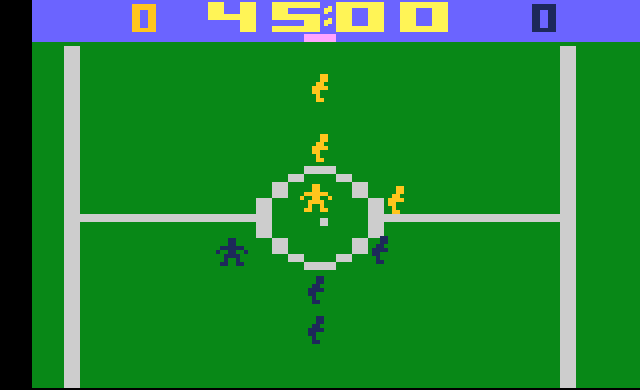
\includegraphics[height=40mm]{imagenes/capitulo1/evofutbol1.png}
	}
	\subfloat[Gol! '92]{
	          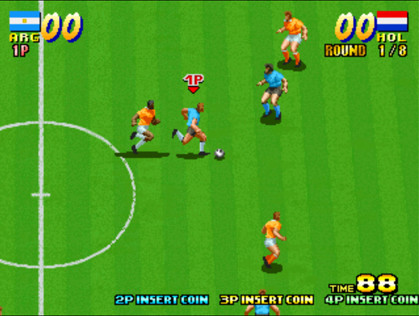
\includegraphics[height=40mm]{imagenes/capitulo1/evofutbol2.jpg}
	}
	\newline
	\subfloat[PES 2012]{
	          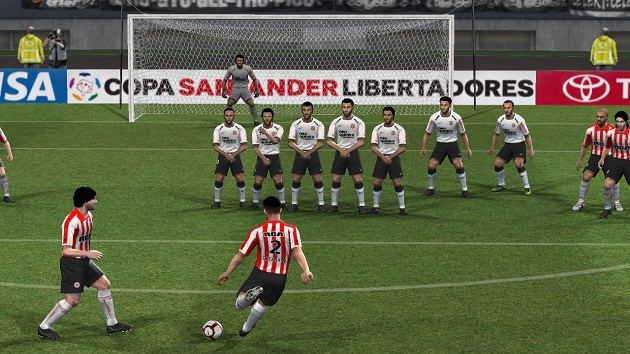
\includegraphics[height=45mm]{imagenes/capitulo1/evofutbol3.jpg}
	}
	\caption{Evolución gráfica en los videojuegos de fútbol}
\end{figure}

Ahora que el videojuego ha captado nuestra atención gráficamente, prestamos atención a la trama que se va entrelazando según avanzamos en él. En los primeros videojuegos la \textbf{historia} desarrollada era nimia pero, poco a poco, éste factor ha ganado importancia, hasta el punto en el cual podemos decir que los costes de desarrollo de un videojuego son equiparables al de una película.
\newline

Existe una característica que pasa desapercibida por el jugador al interiorizarla como algo natural. Estamos hablando de las  \textbf{propiedades físicas} del escenario en el cual nos movemos. El jugador no se para a pensar porqué el personaje que está manejando puede saltar, puede coger otros objetos pero no puede atravesar las paredes. Sin embargo, cuando la física del videojuego no funciona a la perfección, como por ejemplo cuando se atraviesan ligeramente ciertos objetos, no ve el agua de un rio fluir o las llamas del fuego no se mueven, son captadas por el usuario como fallos de importancia. Al igual que el aspecto gráfico de un videojuego, la física esta relacionada con la capacidad de procesamiento. Hoy en día podemos ver juegos que aplican algoritmos para calcular cómo han de moverse los elementos sólidos y fluidos, dando un gran realismo a los juegos.
\newline 

En el transcurso del videojuego podemos encontramos frente a otros personajes, que se relacionan en el escenario, como si fueran manejados por terceras personas. Es la \textbf{inteligencia artificial} la responsable de este comportamiento, que maneja personajes dotándoles de un comportamiento natural, como por ejemplo que un perro persiga y ladre a un extraño o que la gente de tu alrededor te mire si rompes algo. 
\newline

Es sorprendente la evolución de la inteligencia artificial, al principio los movimientos de los personajes podrían catalogarse de burdos y hoy en día nos hace dudar si tras un personaje se encuentra una persona o no.
\newline

Una de las preguntas habituales que todos nos hacemos de forma natural es cómo compartir las experiencias. Existen videojuegos en los cuales no es posible, en otros puede haber varios jugadores simultáneos. Al principio para que se pudiera dar esta situación, había que estar en la misma sala, sin embargo esta limitación desapareció debido a la \textbf{conectividad} de los soportes a través de Internet. Esta característica ha llevado a los videojuegos a un nuevo nivel convirtiéndolos en un acto social.

\subsection{Videojuegos en dispositivos móviles}

Una vez descrita la evolución de los videojuegos, tanto a niveles de formatos como características, se van a describir las implicaciones en el ámbito de los smartphone. 

\begin{figure}[h]
	\centerfloat	 
	\subfloat[Apalabrados]{
	          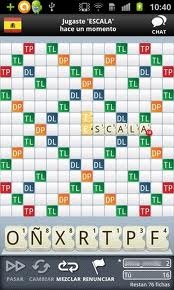
\includegraphics[height=60mm]{imagenes/capitulo1/apalabrados.jpg}
	}
	\subfloat[Angry Birds]{
	          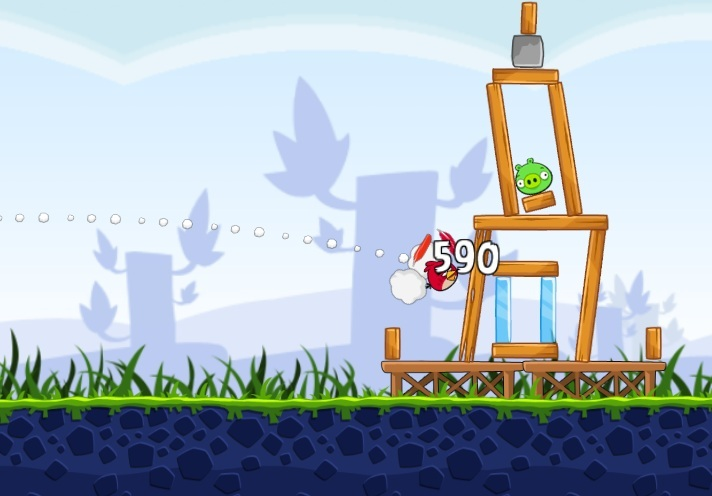
\includegraphics[height=50mm]{imagenes/capitulo1/angrybirds.jpg}
	}
	\subfloat[Candy Crush Saga]{
	          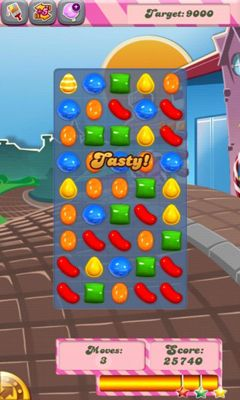
\includegraphics[height=60mm]{imagenes/capitulo1/candycrush.jpg}
	}
	\caption{Top éxitos en Android}
\end{figure}

A pesar de la gran evolución de los móviles, su capacidad de procesamiento no es, ni de lejos, comparable con las computadoras de sobremesa ni consolas. A esta situación se le suma un mercado emergente y que no dispone de frameworks especializados para el desarrollo de videojuegos, lo que ha provocado una involución en casi todas sus características.
Este hecho puede constatarse al consultar los videojuegos más descargados para Android. Predominan los juegos sin una historia desarrollada y con un aspecto visual simplista. Alguno de ellos son Apalabrados, Candy Crush Saga y Angry Bird, de los cuales se muestran capturas de pantalla en la figura 1.6.
\newline

Un ejemplo de un videojuego que aprovecha el potencial de los smarthones actuales es el Grand Theft Auto, a pesar de ello, existe una gran diferencia en su aspecto gráfico en comparación con la versión de consola, tal y como muestran las siguientes capturas de pantallas.

\begin{figure}[h]
	\centerfloat	 
	\subfloat[Android/iPhone]{
	          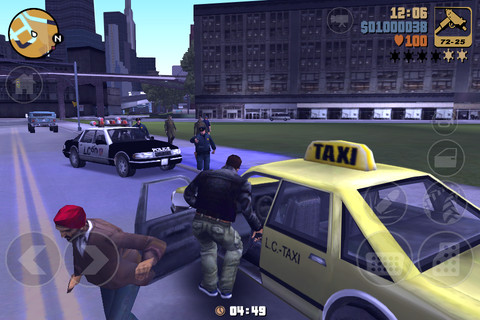
\includegraphics[height=45mm]{imagenes/capitulo1/GTA3.jpg}
	}
	\subfloat[Play Station 3]{
	          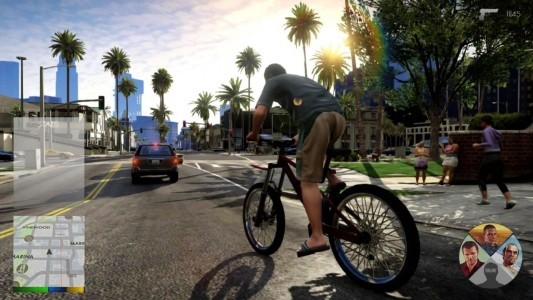
\includegraphics[height=45mm]{imagenes/capitulo1/GTAV.jpg}
	}
	\caption{Grand Theft Auto}
\end{figure}

Una dificultad añadida consiste en la desaparición del teclado y mandos con los que controlar el videojuego, siendo sustituida en la mayoría de los casos por la pantalla táctil o lo sensores de movimiento del dispositivo. 
\newline

Hay que destacar que un smartphone ofrece un serie de características adicionales propias de ellos, la más destacables son el GPS y la cámara. De estas cualidades han surgido dos conceptos nuevos:
\begin{itemize}
\item La \textbf{movilidad} permite a las aplicaciones mejorar su funcionamiento al poder incluir la posición en la que nos encontramos. Por ejemplo, nos permite saber cúal es la estación de metro más cercana o hacer campañas publicitarias por proximidad.
\item La \textbf{realidad aumentada} permite mezclar el mundo real y el digital a través del uso de la cámara. Por ejemplo, podríamos ver como nos queda un mueble en un salón a través de la cámara.
\end{itemize}

\begin{figure}[h]
	\centerfloat	 
        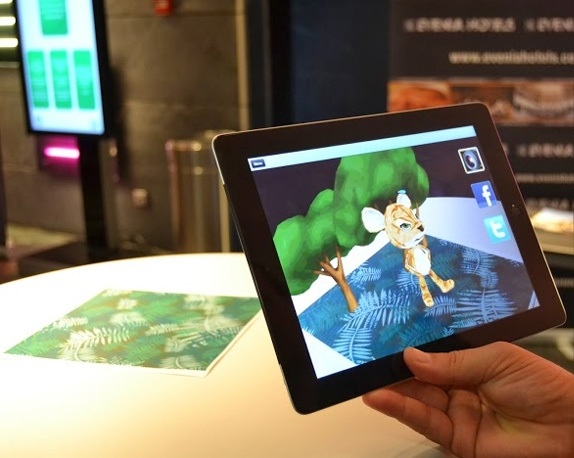
\includegraphics[height=45mm]{imagenes/capitulo1/realidadaumentada.jpg}
	\caption{Ejemplo de realidad aumentada}
\end{figure}

Éstas particularidades están estimulando la creación de otros tipos de videojuegos, como por ejemplo Ingress, de Google. Este videojuego consiste en salir a la calle con el móvil, abrir la aplicación y buscar  \emph{fuentes de esta misteriosa energía} ocultas en nuestra ciudad, transformando el mundo real en el escenario del videojuego mediante el uso de las la cámara, las redes de telefonía y el GPS. 
%\newline
%
%Visto desde perspectivas comerciales, este tipo de videojuegos pueden ser utilizados para recoger una cantidad ingente de información de %geoposicionamiento, la cúal puede ser utilizada para mejorar Google Maps con la ayuda de todos.

\section{Objetivos del proyecto}

Una vez explicadas las motivaciones que han dado lugar al proyecto de fin de carrera, la evolución de los videojuegos y la implicaciones que existentes en smartphone, se van a definir los objetivos del proyecto.

\begin{enumerate}
\item Adquirir los conocimientos específicos necesarios para poder desarrollar videojuegos con modelos en 3D.
\item Aprender a realizar diseños gráficos con Blender para generar el aspecto gráfico de los elementos de un videojuego.
\item Aprender el lenguaje de programación específico para tarjetas gráficas llamado GLSL (OpenGL Shading Language).
\item Conseguir los conocimientos del desarrollo de aplicaciones en Android.
\item Comprar un smarthpone adecuado para el desarrollo del proyecto que cuente con el hardware que permita aceleración gráfica mediante OpenGL ES 2.0 y la versión Gingerbread de Android. Estos conceptos son desarrollos en la primera parte del proyecto. Tras realizar un estudio de mercado de los smarthpone que cubrían esta características, el móvil elegido fue el HTC Desire.
\item Desarrollar una librería genérica que facilite el desarrollo de videojuegos para Android. La llamaremos TfcGameEngine y contendrá diversas funcionalidades:
	\begin{itemize}
	\item Bucle principal del videojuego en el cual se van secuenciando imágenes como si de una película se tratase.
	\item Soporte para OpenGL ES 2.0 (Este concepto que se explicará en el capítulo 3 del proyecto).
	\item Utilidades para el cálculo de movimiento en función del tiempo, velocidad y aceleración, es decir, cinemática.
	\item Detección de colisiones entre elementos del juego.
	\item Algoritmos que permitan desplazar los personajes de videojuego sobre la escena de forma manual, aleatoria o entre dos puntos.
	\item Procesamiento de los diseños gráficos realizados con Blender.
	\item Motor de música que permita reproducir melodías y efectos de sonido.
	\end{itemize}

	Un principio básico que ha primado en el diseño de la librería es que tiene que ser fácilmente extensible por terceros, permitiendo de esta forma, añadir nuevas funcionalidades. 

\item Realizar una prueba de concepto de dicha librería programando un videojuego de un comecocos en 3D, llamado Pacmania. Este juego consiste en controlar al Pacman, un personaje que ha de recoger las pastillas de un escenario custodiado por fantasmas. Para ello será necesario:
	\begin{itemize}
	\item Realizar los diseños gráficos de los escenarios y personajes del videojuego, que son dos escenarios, un fantasma y un pacman.
	\item Realizar un proceso de carga de los ficheros contenidos en un directorio de configuración. Este directorio contiene los escenarios, personajes, efectos especiales, melodías, vídeos, etc.
	\item Ampliación de la librería TfcGameEngine para incluir la lógica especifica del videojuego como por ejemplo, controlar la puntuación y número de vidas de la partida.
	\item Creación de animaciones con la cámara cuándo comienza un nivel o el Pacman es capturado por un fantasma.
	\item Reproducción de efectos especiales y melodías.
	\item Pantalla de configuración que permita indicar si el sonido esta activo y donde se encuentra el directorio de configuración.
	\item Registro de las mejores puntuaciones en una base de datos SqlLite.
	\end{itemize}
\item Testar el videojuego en otros smartphone como Galaxy S2 y Nexus 5.
\end{enumerate}

Para mas información sobre la librería TfcGameEngine y el juego Pacmania, consultar los catálogo de requisitos del capítulo 5.